%
\chapter{Projeto C}

Neste projeto construímos uma rede com dois nós. O primeiro nó contem dois sensores e o segundo nó contem um LED atuador. O nó contendo os sensores apresenta dois sensores um DTH11 para coletar informações de temperatura e umidade e um sensor LDR para monitor a luminosidade do ambiente. Este projeto possui o intuito de apresentar ao leitor o funcionamento de um nó com mais de um sensor e apresentar também um nó atuador. 
Vamos construir um nó sensor para coletar informações de temperatura, umidade e luminosidade e outro nó para emitir um sinal de alerta dependendo das informações dos sensores, os dois nós devem se comunicar com o controlador.

\section{Materiais}

Para esse projeto vamos o utilizar os seguintes materiais:
\begin{itemize}
\item 3 Arduinos;
\item Sensor de temperatura e umidade DTH11;
\item Sensor de luminosidade LDR;
\item LED;
\item Resistor 220 ohms;
\item 3 Rádios nRF24L01;
\item Jumpers;
\item Protoboard.
\end{itemize}

Para obter mais informações sobre os materiais consulte o capitulo ~\ref{MateSof}.

\section{Implementação}

\subsection{Gateway}
\vbox{
\indent \rule{10.4cm}{0.6pt}\par
\textbf{Esquemático}\par%\vspace{-0.66\baselineskip}
\rule[0.90\baselineskip]{10.4cm}{0.6pt}
}

\begin{figure}[ht]
      \centering
      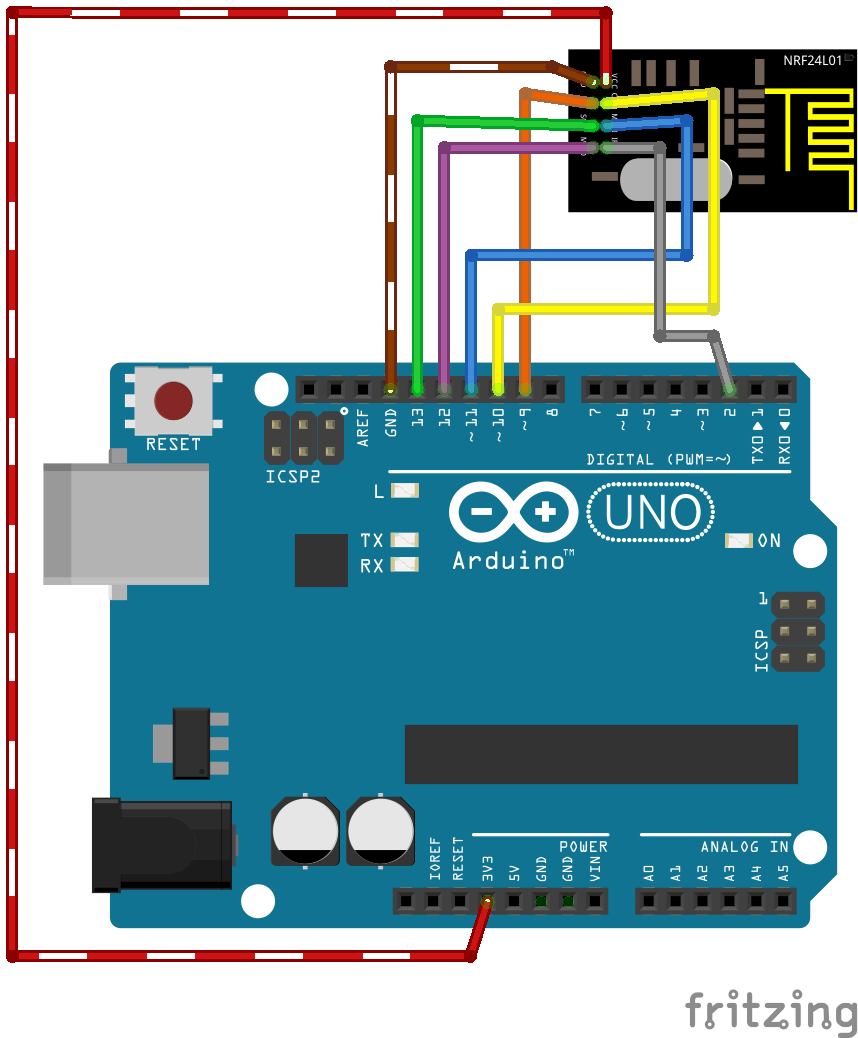
\includegraphics[scale=0.70]{figuras/gateway.png}
      \caption{Gateway}
      \label{fig:gateway3}
\end{figure}
\pagebreak
\vbox{
\indent \rule{10.4cm}{0.6pt}\par
\textbf{Código}\par%\vspace{-0.66\baselineskip}
\rule[0.90\baselineskip]{10.4cm}{0.6pt}
}

\lstinputlisting[language=C++, caption={Gateway}]{code/teste.ino}

\subsection{Nó com sensor DTH11 e LDR}

\vbox{
\indent \rule{10.4cm}{0.6pt}\par
\textbf{Esquemático}\par%\vspace{-0.66\baselineskip}
\rule[0.90\baselineskip]{10.4cm}{0.6pt}
}

\begin{figure}[ht]
      \centering
      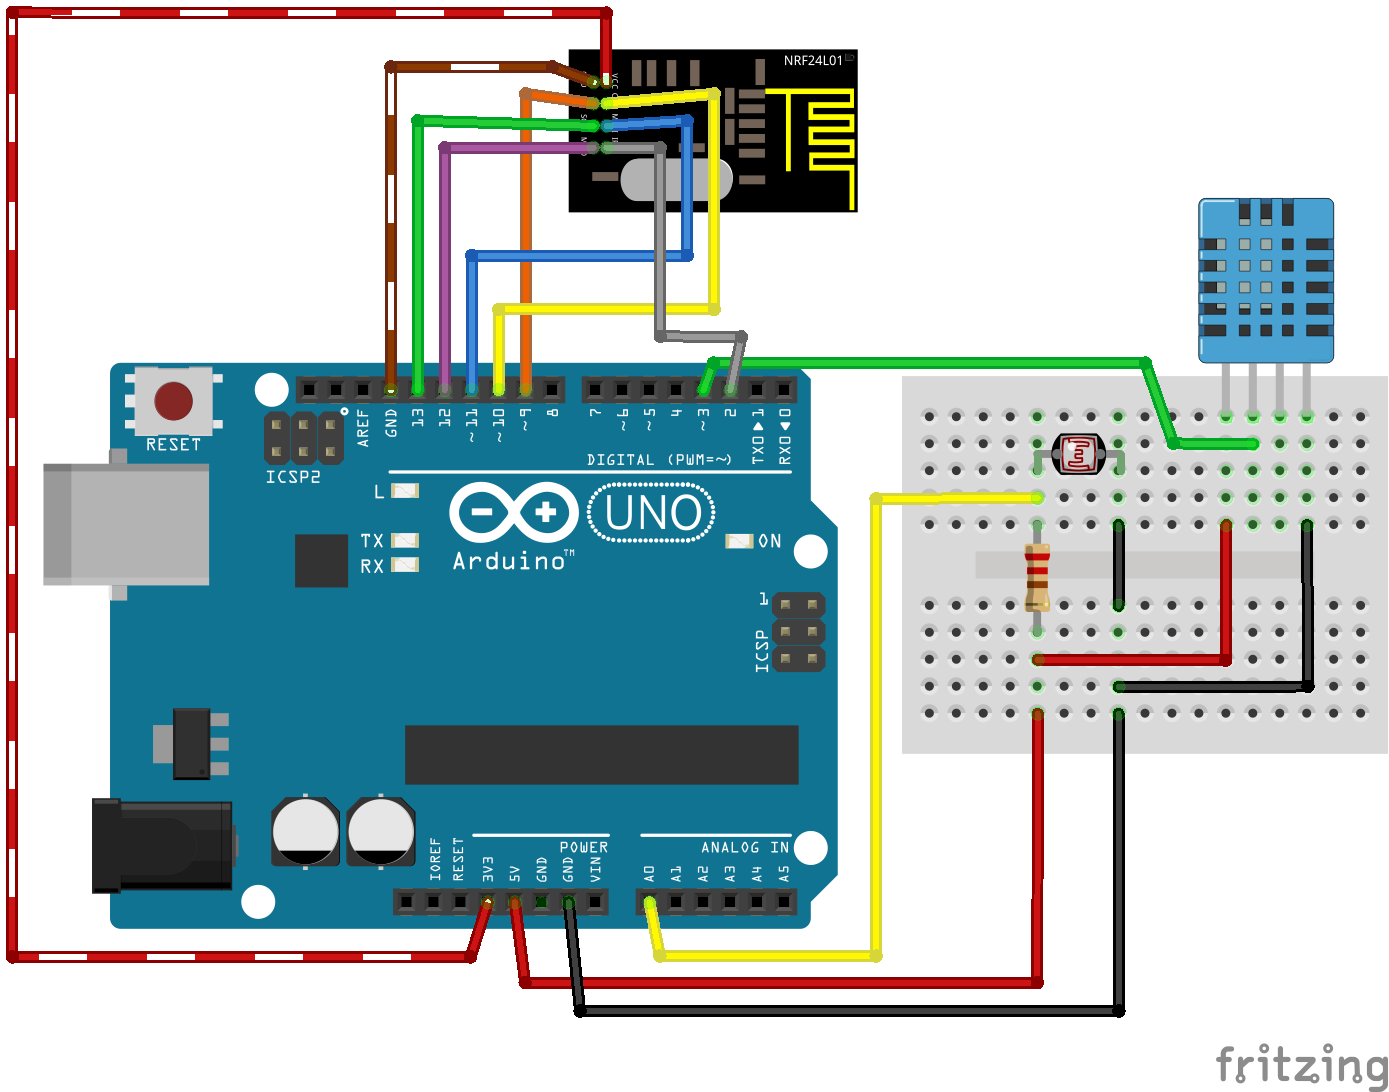
\includegraphics[scale=0.70]{figuras/ldrPdth11_bb.png}
      \caption{Nó Sensor DTH11 e LDR}
      \label{fig:dth11ldr}
\end{figure}
\pagebreak
\vbox{
\indent \rule{10.4cm}{0.6pt}\par
\textbf{Código}\par%\vspace{-0.66\baselineskip}
\rule[0.90\baselineskip]{10.4cm}{0.6pt}
}

\lstinputlisting[language=C++, caption={LDR e DTH11 }]{code/ldr_dth11.ino}


\subsection{Nó com atuador LED}

\vbox{
\indent \rule{10.4cm}{0.6pt}\par
\textbf{Esquemático}\par%\vspace{-0.66\baselineskip}
\rule[0.90\baselineskip]{10.4cm}{0.6pt}
}

\begin{figure}[ht]
      \centering
      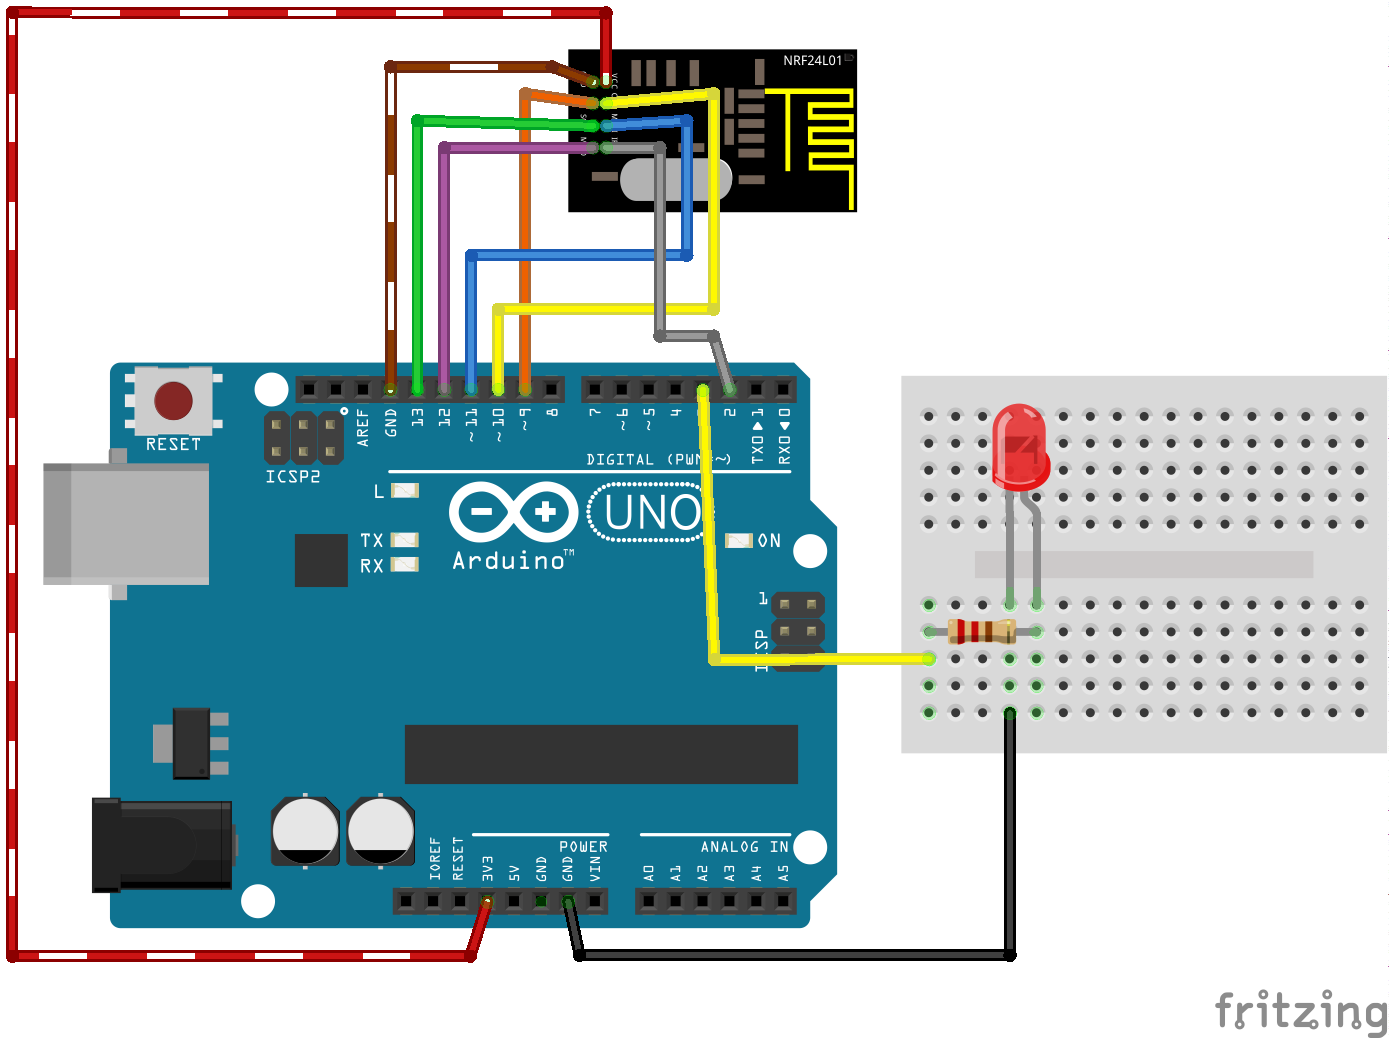
\includegraphics[scale=0.70]{figuras/led_bb.png}
      \caption{Nó LED}
      \label{fig:led}
\end{figure}
\pagebreak
\vbox{
\indent \rule{10.4cm}{0.6pt}\par
\textbf{Código}\par%\vspace{-0.66\baselineskip}
\rule[0.90\baselineskip]{10.4cm}{0.6pt}
}

\lstinputlisting[language=C++, caption={LED}]{code/led.ino}


\subsection{Controlador}

Arquivo de configuração do Pimatic

\lstinputlisting[language=C++, caption={json.conf}]{code/jsonC.json}